Here's the updated LaTeX code, with the figures integrated and captions updated. I've used X.Y as placeholders for chapter and figure numbers, as requested, and made sure the image paths are correct.

Generated latex
\section{Platform Features}
This section provides a comprehensive overview of the data annotation platform's features, highlighting its core functionalities, architectural design principles, and collaborative capabilities. The design emphasizes modularity, scalability, and an intuitive user experience, while leveraging a robust backend for automated processes.

\subsection{Authorization and Access Control}
The platform incorporates a sophisticated authorization system designed for granular control over resources and actions, ensuring data security and user privacy.

\subsubsection{Attribute-Based Access Control (ABAC)}
Instead of rigid, static roles, the system employs Attribute-Based Access Control (ABAC). Permissions are dynamically evaluated based on various attributes, including those of the user (e.g., role within a project), the resource (e.g., project, task, assignment), and the specific action being attempted (e.g., `create`, `delete`, `comment`). This enables highly flexible and fine-grained security policies.

\subsubsection{Contextual and Secure Authentication}
Access decisions are inherently contextual, with user permissions determined by their specific role within a given project. User authentication is securely managed through Supabase Auth, and user profiles store additional attributes (e.g., full name, avatar) that can further inform access control policies.

\begin{figure}[h!]
    \centering
    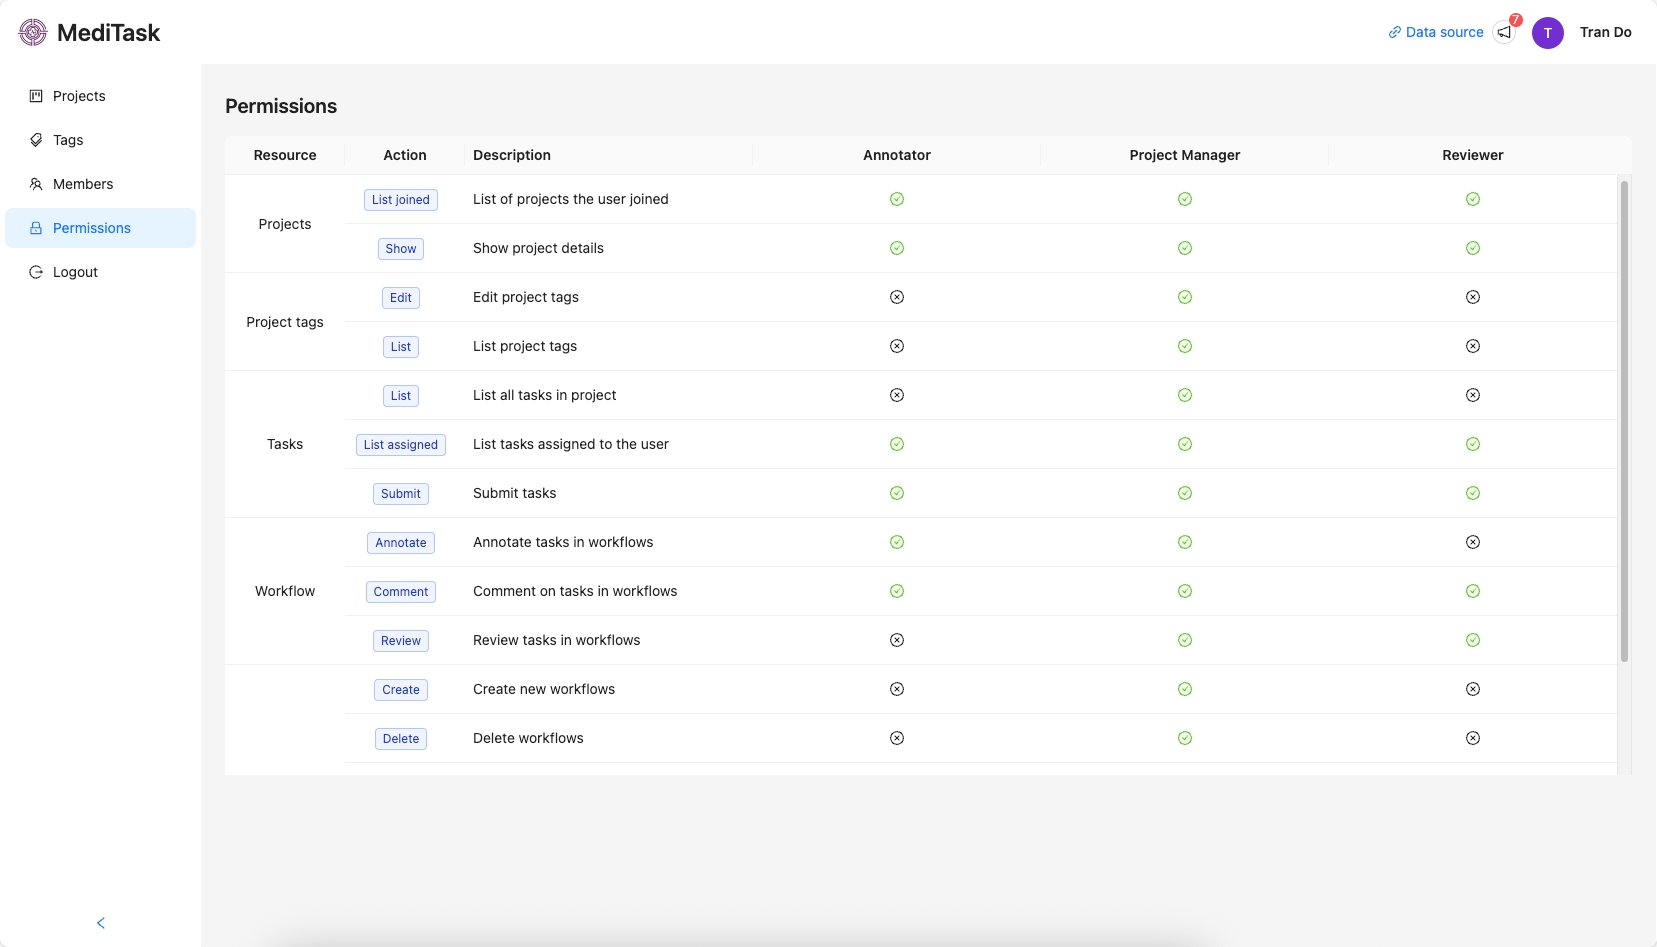
\includegraphics[width=1\textwidth]{content//resources//features//permissions.png}
    \caption{Granular Permissions Configuration Interface}
    \label{fig:permissions-config}
\end{figure}

\subsection{Workflow Management}
At the heart of the platform lies a powerful and adaptable workflow engine that facilitates the construction and execution of complex data processing pipelines.

\subsubsection{Dynamic Workflow Graphs}
Workflows are visually represented and defined as directed graphs, comprising interconnected stages (nodes) and connections (edges). This graph structure is customizable per project, allowing for bespoke data processing flows. Figure~\ref{fig:workflow-editor-simple} illustrates the intuitive drag-and-drop interface for designing workflows, while Figure~\ref{fig:workflow-editor-advanced} demonstrates a more complex workflow incorporating routing and consensus stages.

\begin{figure}[h!]
    \centering
    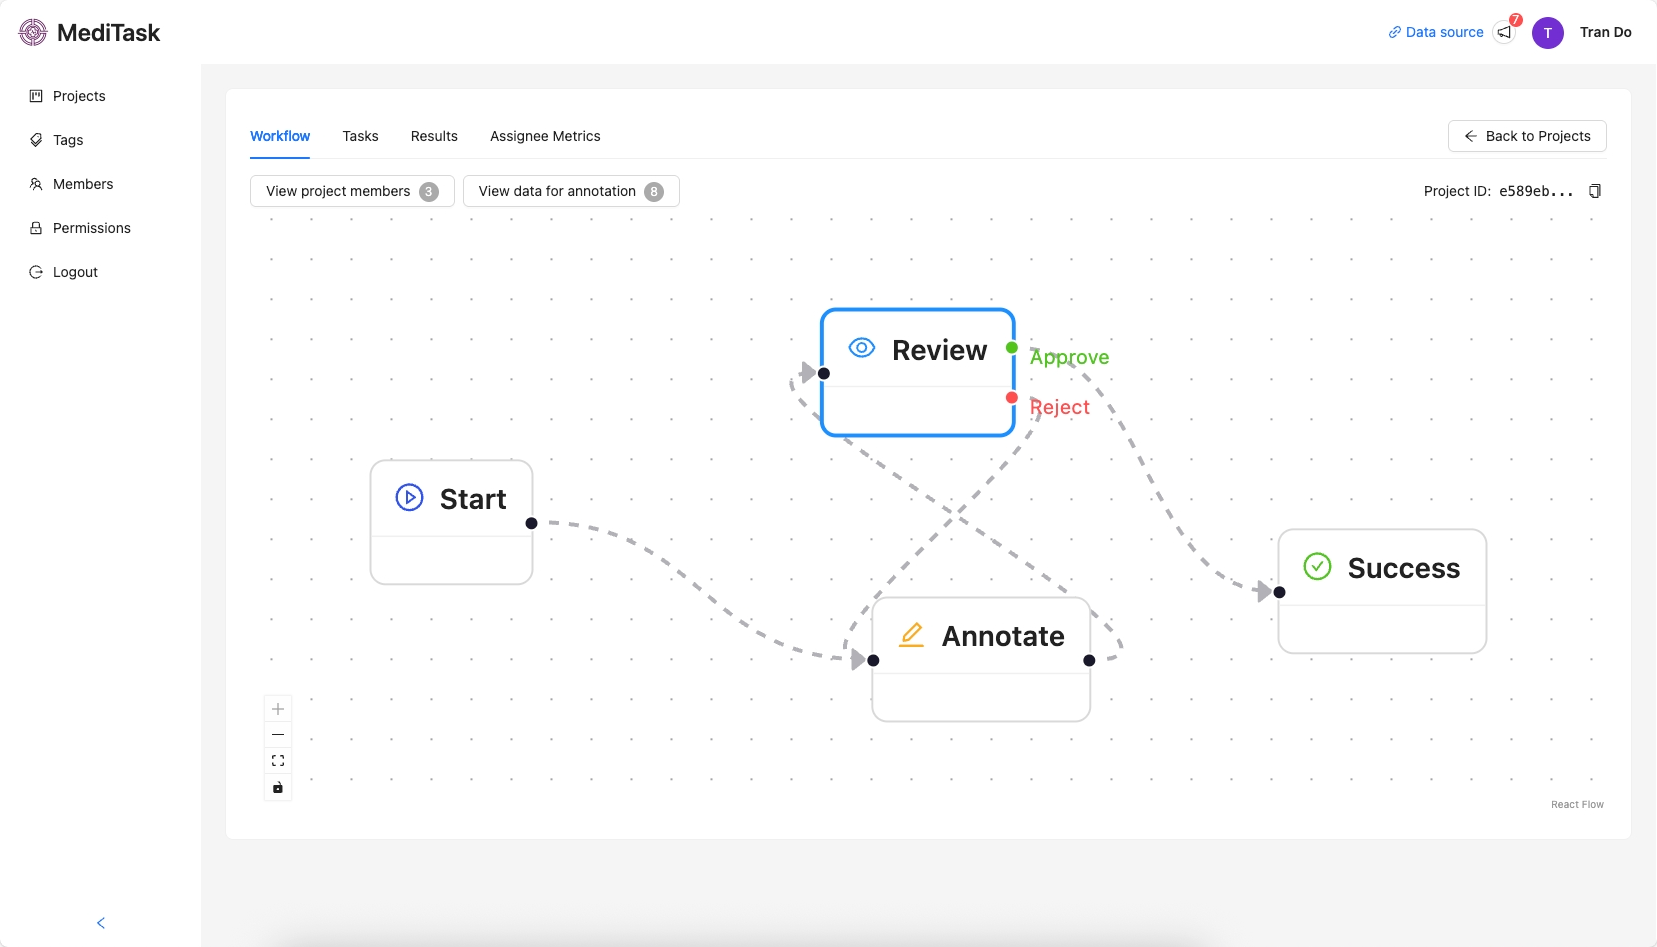
\includegraphics[width=1\textwidth]{content/resources/features/simple workflow.png}
    \caption{Workflow Design Interface}
    \label{fig:workflow-editor-simple}
\end{figure}

\begin{figure}[h!]
    \centering
    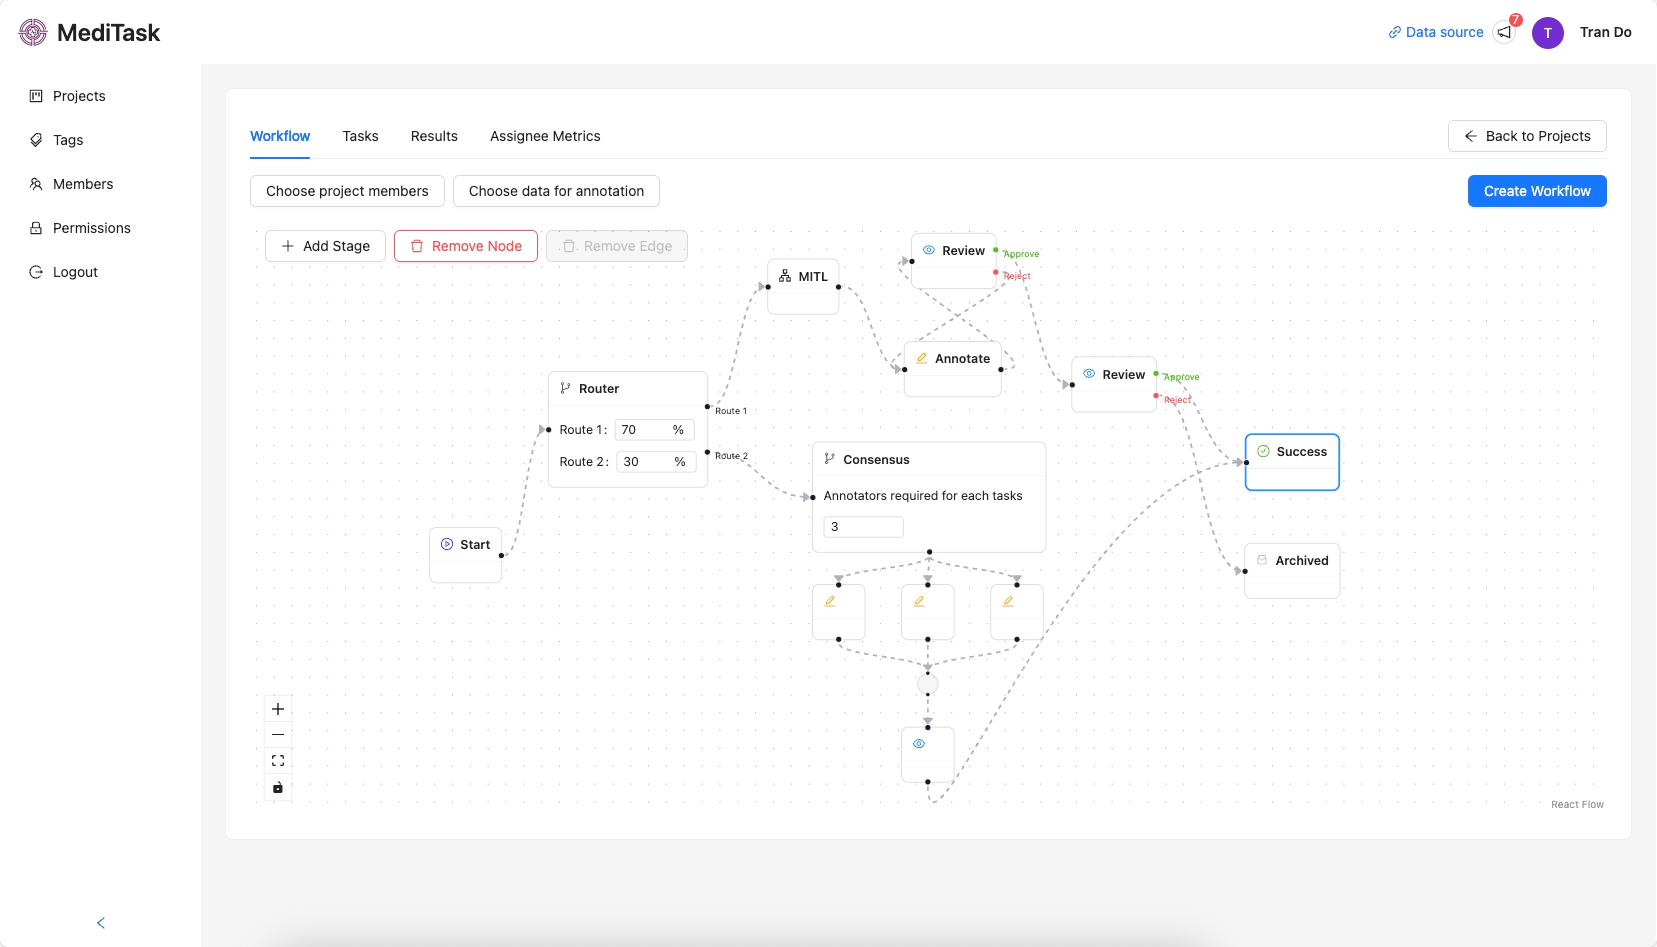
\includegraphics[width=1\textwidth]{content/resources/features/complex workflow.png}
    \caption{Advanced Workflow with Router and Consensus Stages}
    \label{fig:workflow-editor-advanced}
\end{figure}

\subsubsection{Customizable Stages and Conditional Logic}
Each workflow stage possesses a distinct type (e.g., \texttt{ANNOTATE}, \texttt{REVIEW}, \texttt{CONSENSUS}) and can host unique custom configurations. The system supports advanced conditional branching, enabling distinct success and failure paths for tasks at each stage, ensuring resilient workflow progression. As shown in Figure~\ref{fig:workflow-select-members}, users can easily select project members and their roles, which can then be assigned to workflow stages.

\begin{figure}[h!]
    \centering
    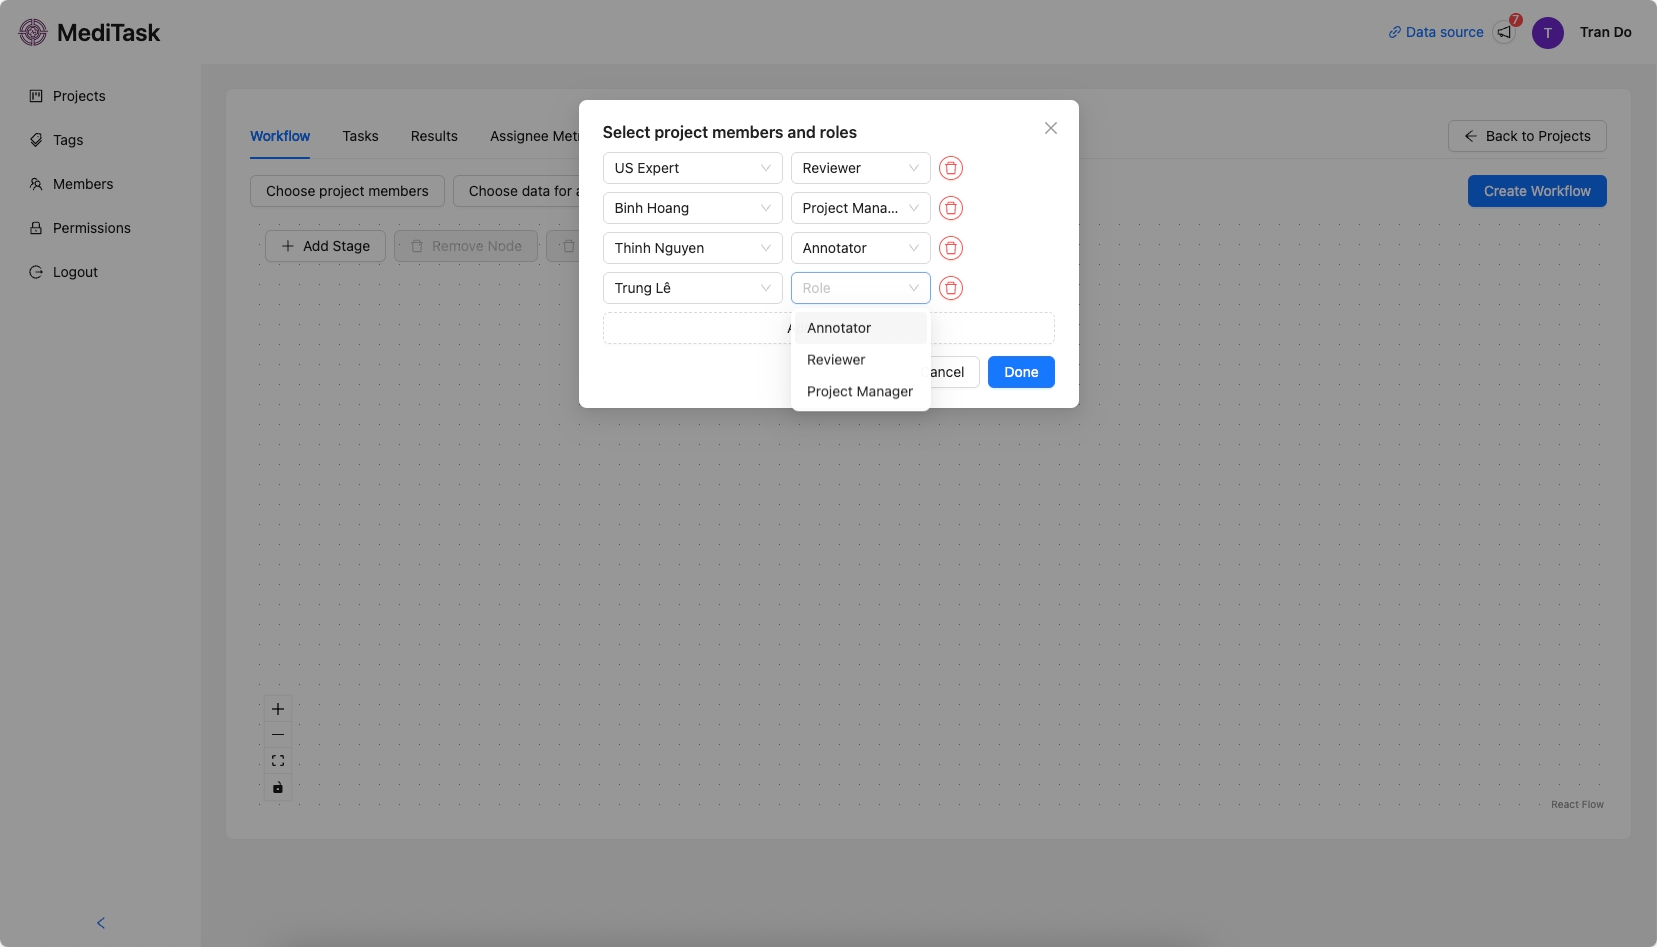
\includegraphics[width=0.6\textwidth]{content/resources/features/choose members.png}
    \caption{Selecting Project Members for Workflow Assignment}
    \label{fig:workflow-select-members}
\end{figure}

\subsubsection{Automated Assignee Selection}
The platform can automatically determine the subsequent assignee for a task based on functions linked to each workflow stage. This capability underpins complex routing logic, optimizing task distribution and flow. Figure~\ref{fig:workflow-select-data} demonstrates the process of selecting specific data instances to be included in a workflow, ensuring only relevant data undergoes the defined process.

\begin{figure}[h!]
    \centering
    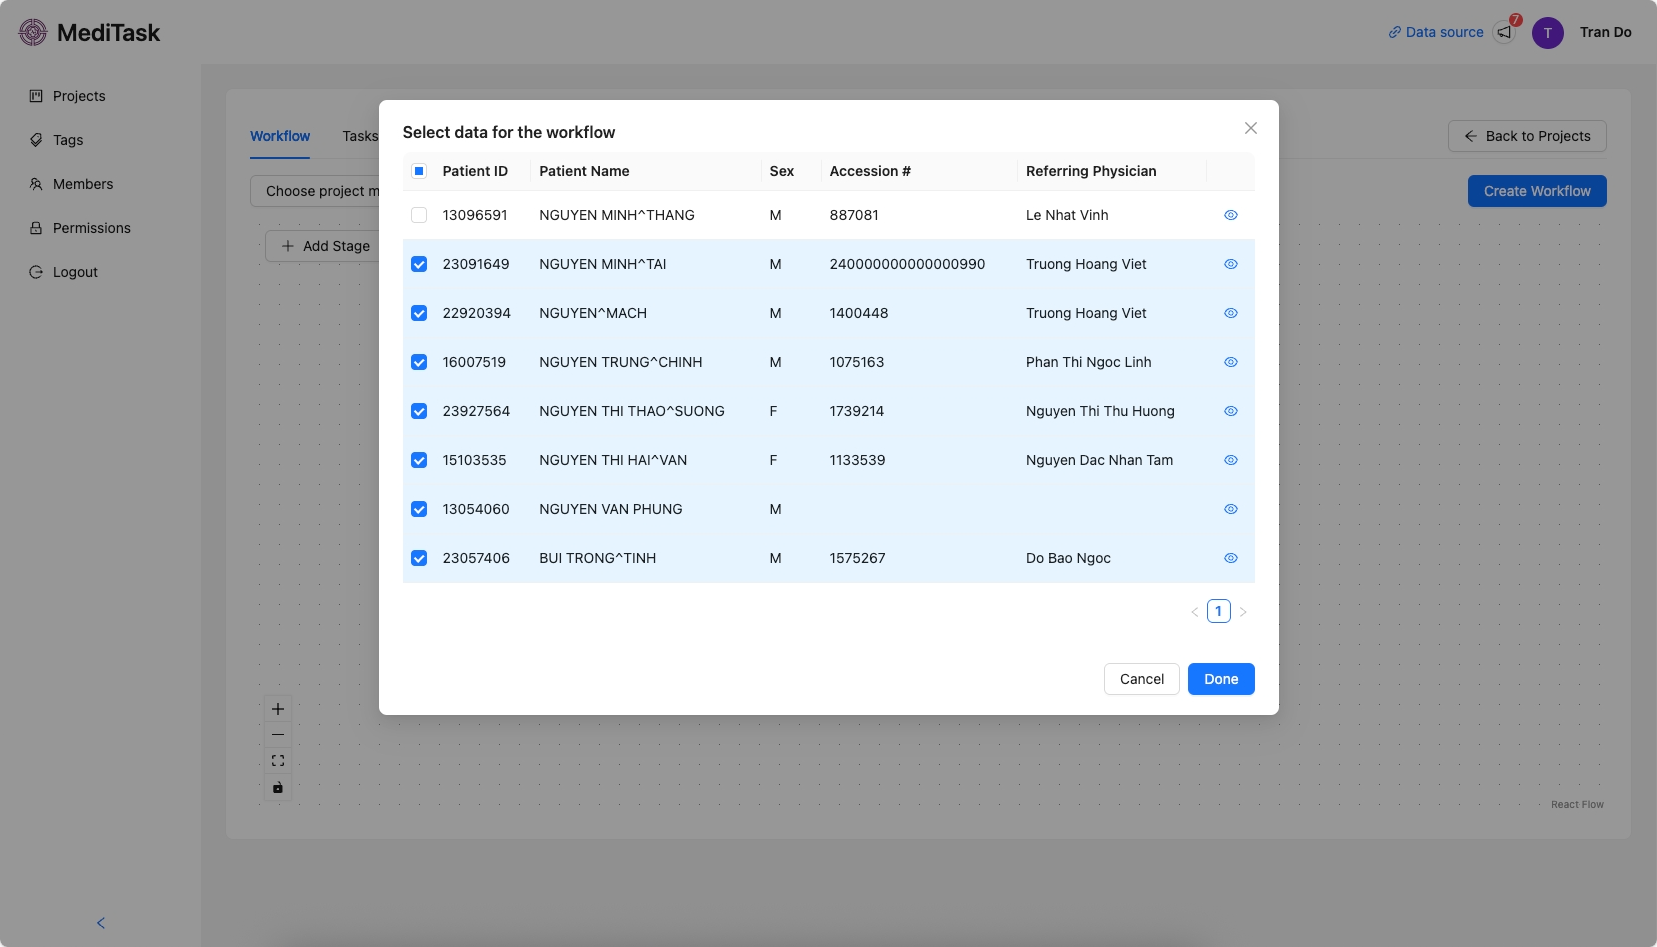
\includegraphics[width=0.6\textwidth]{content/resources/features/choose dataset.png}
    \caption{Selecting Data Instances for Workflow Processing}
    \label{fig:workflow-select-data}
\end{figure}

\subsection{Project \& Task Management}
Comprehensive tools are provided for the organization and management of projects and their constituent tasks.

\subsubsection{Centralized Project Hub}
Projects serve as the primary organizational unit, encapsulating datasets, tasks, and member assignments. Each project is defined by a name, description, and an associated set of members, providing a consolidated view for all related activities. Figure~\ref{fig:project-list} illustrates the centralized project hub, allowing users to overview and manage their ongoing annotation efforts. Projects can also be categorized using a flexible, color-coded tagging system, enhancing visual identification and search capabilities, as seen in Figure~\ref{fig:tags-list}.

\begin{figure}[h!]
    \centering
    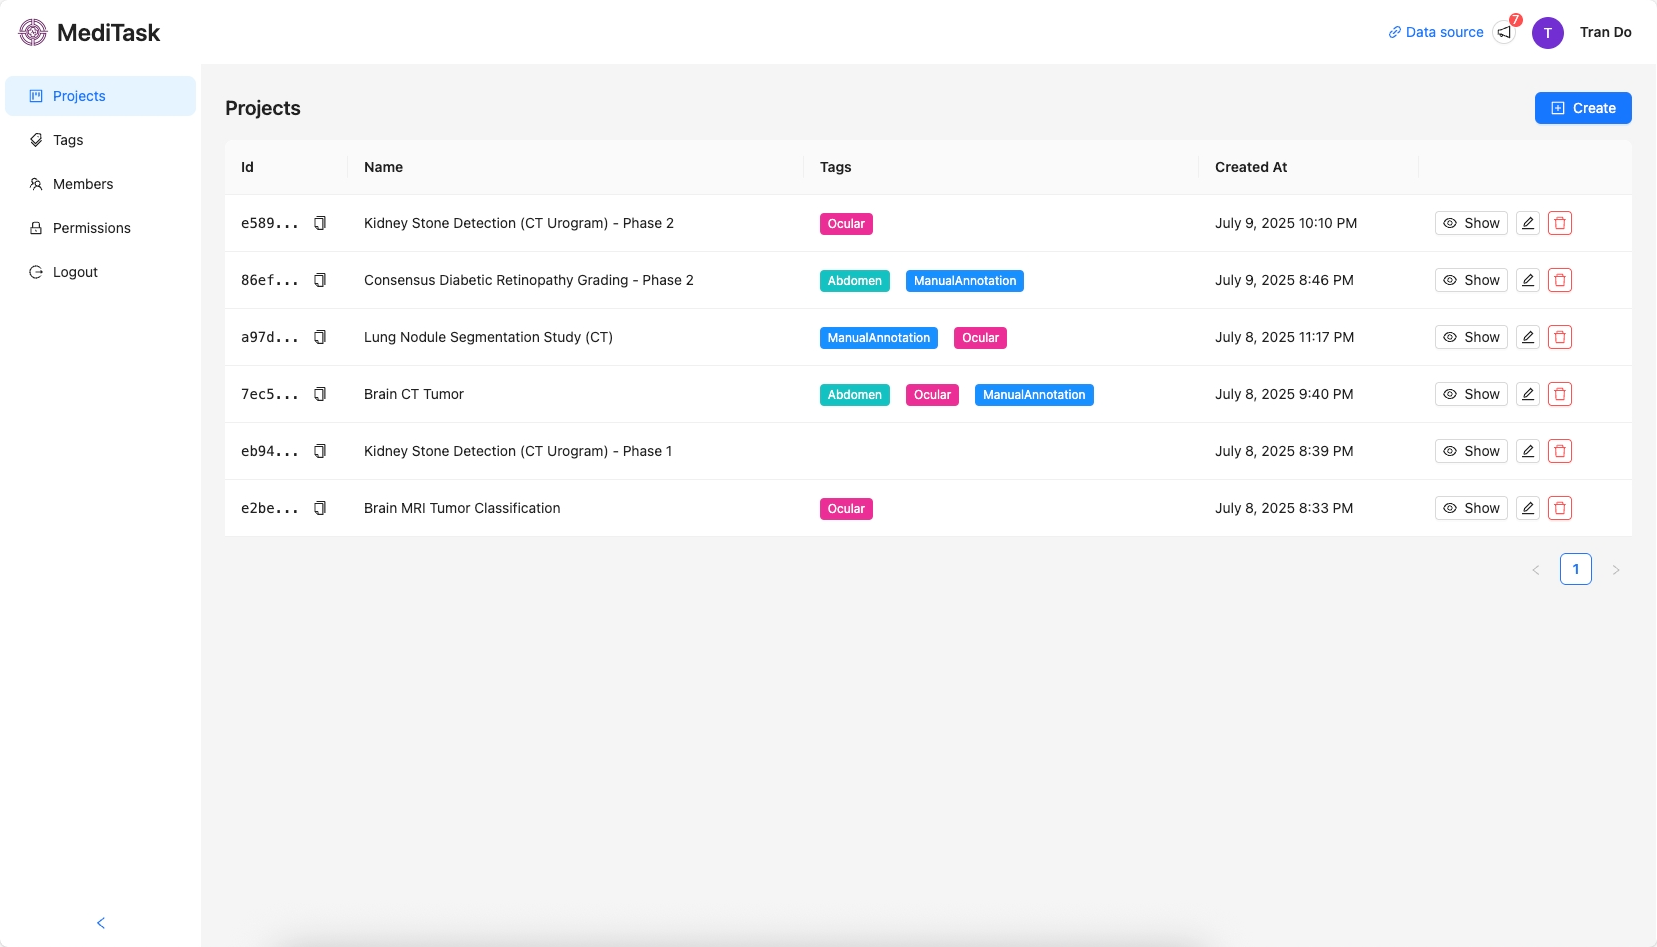
\includegraphics[width=1\textwidth]{content//resources//features//projects.png}
    \caption{Layout of Project Management Page}
    \label{fig:project-list}
\end{figure}

\begin{figure}[h!]
    \centering
    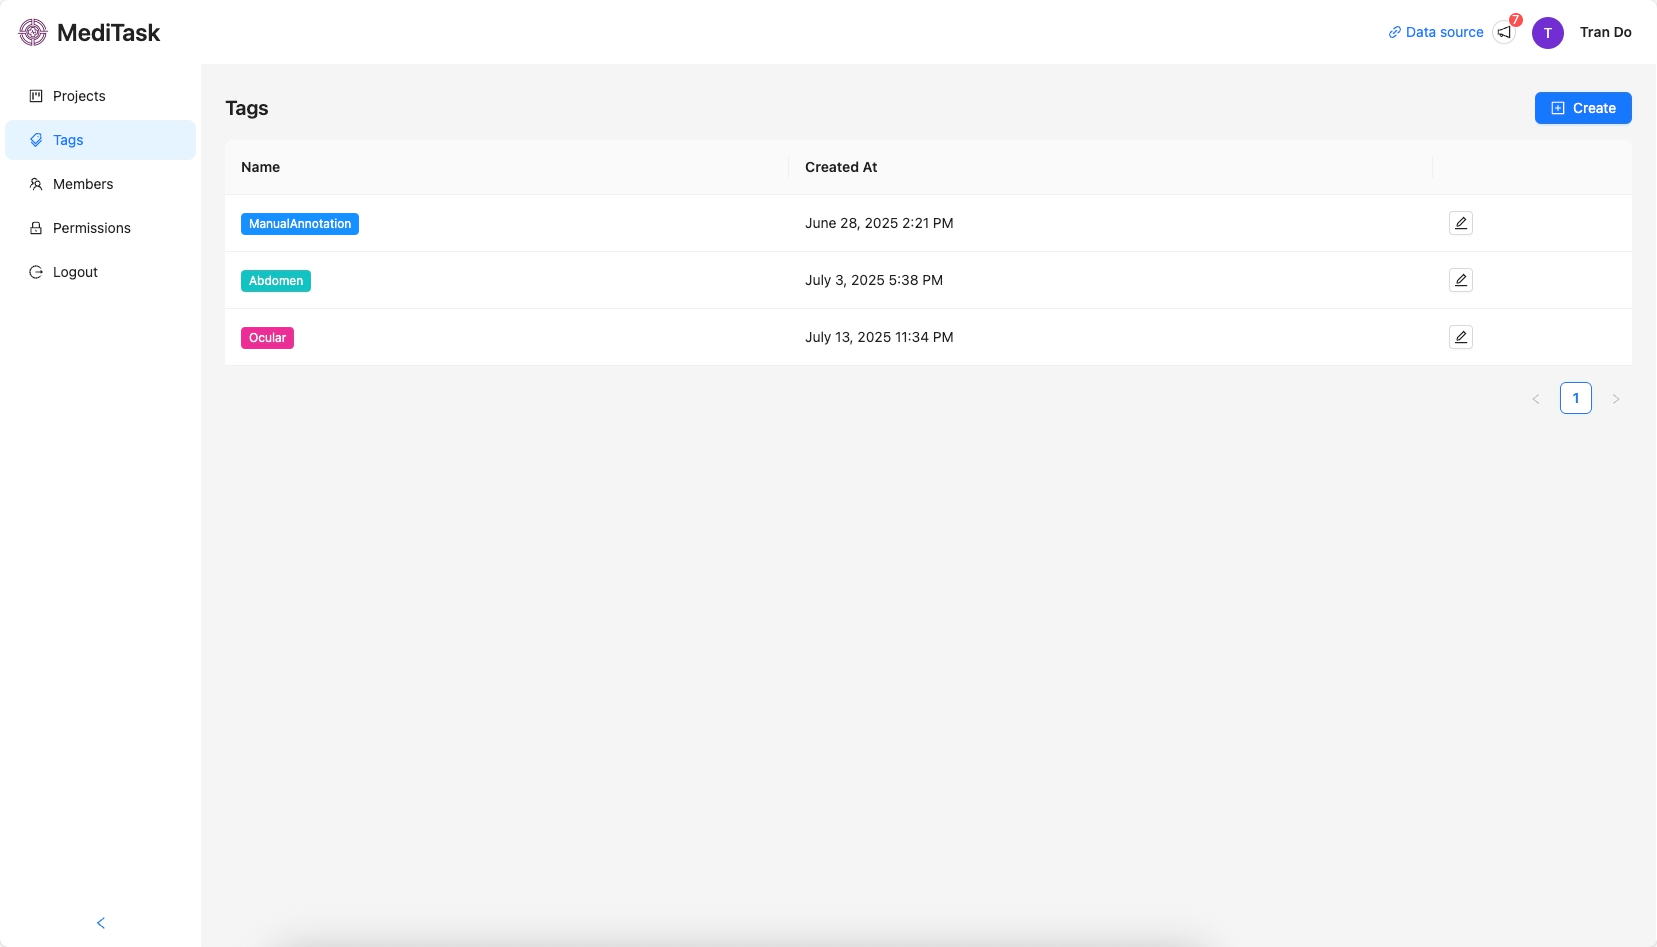
\includegraphics[width=1\textwidth]{content//resources//features//tags.png}
    \caption{Project Tag Management Interface}
    \label{fig:tags-list}
\end{figure}

\subsubsection{Task Lifecycle Management}
Tasks represent discrete units of work tied to specific data items. They transition through various statuses (e.g., \texttt{PENDING}, \texttt{COMPLETED}) as they advance through the defined workflow, ensuring clear visibility of progress. Figure~\ref{fig:tags-list} and Figure~\ref{fig:tasks-tab-1} showcase different views of the task list within a project, providing comprehensive oversight of task status, assignment, and progress.

\begin{figure}[h!]
    \centering
    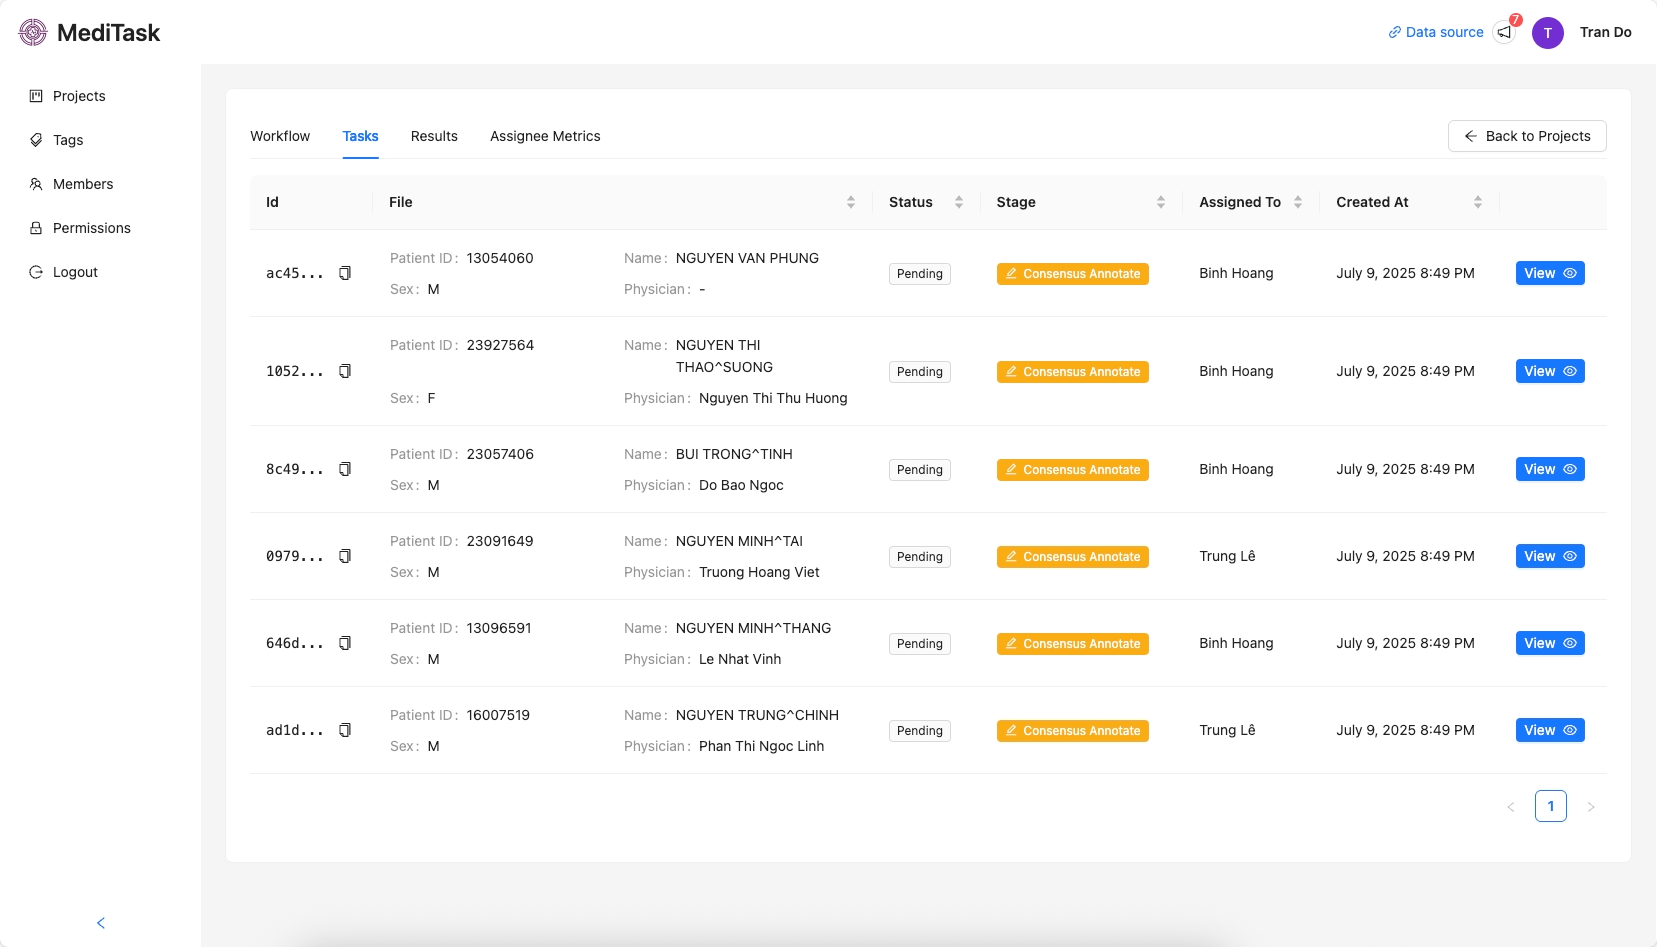
\includegraphics[width=1\textwidth]{content/resources/features/tasks.png}
    \caption{Task List View within a Project}
    \label{fig:tasks-tab-1}
\end{figure}

\subsubsection{Detailed Task Assignments}
Task progression through a workflow is managed via assignments. Each assignment links a task to a specific user at a particular workflow stage, meticulously tracking its status, start time, and completion time, creating an auditable trail.

\subsection{Member Management}
The platform facilitates the effective management of users and their roles within projects.

\subsubsection{User and Project-Level Role Management}
Administrators can create, list, and modify user accounts within the system. Critically, roles are assigned on a per-project basis, allowing for granular control over user permissions and responsibilities tailored to each project's needs. While a dedicated member list view is not shown, the `Permissions` interface (Figure~\ref{fig:permissions-config}) implicitly demonstrates the role-based access control for different user types.

\subsection{Annotation \& Collaboration}
The platform is meticulously designed to foster efficient and accurate data annotation through a robust collaborative environment.

\subsubsection{Integrated Annotation Tools}
The system seamlessly integrates with industry-standard tools such as OHIF Viewer, MONAI, and Orthanc. This integration supports advanced medical imaging annotation workflows and enables AI-assisted labeling functionalities. Figure~\ref{fig:annotation-viewer} provides a view of the integrated medical imaging annotation environment, while Figure~\ref{fig:orthanc-integration} shows the external Orthanc integration for data source management.

\begin{figure}[h!]
    \centering
    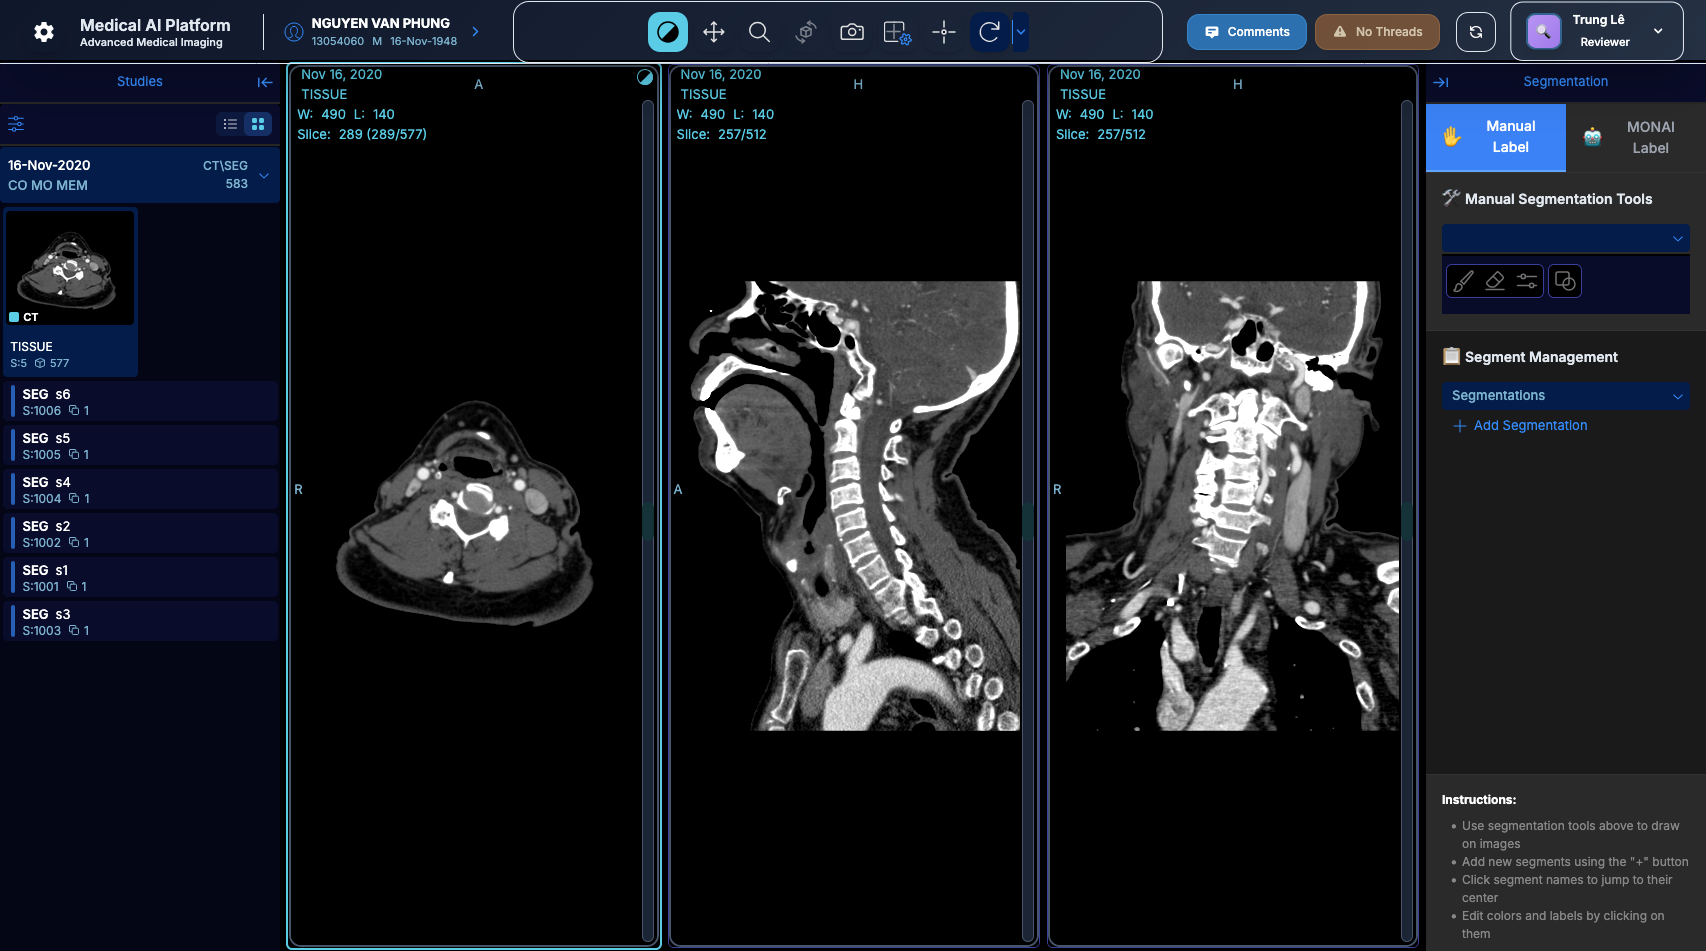
\includegraphics[width=1\textwidth]{content/resources/features/ohif.png}
    \caption{Integrated Medical Imaging Annotation Viewer}
    \label{fig:annotation-viewer}
\end{figure}

\subsubsection{Annotation Commenting and Segmentation Data}
Users can leave rich, structured comments on task assignments, facilitating detailed discussions and feedback loops. Figure~\ref{fig:annotation-comments} illustrates the task assessment hub, which includes a dedicated section for comments and collaboration. Tasks are also capable of storing lists of segmentation IDs, which are crucial for image-based annotation tasks involving precise object boundaries.

\begin{figure}[h!]
    \centering
    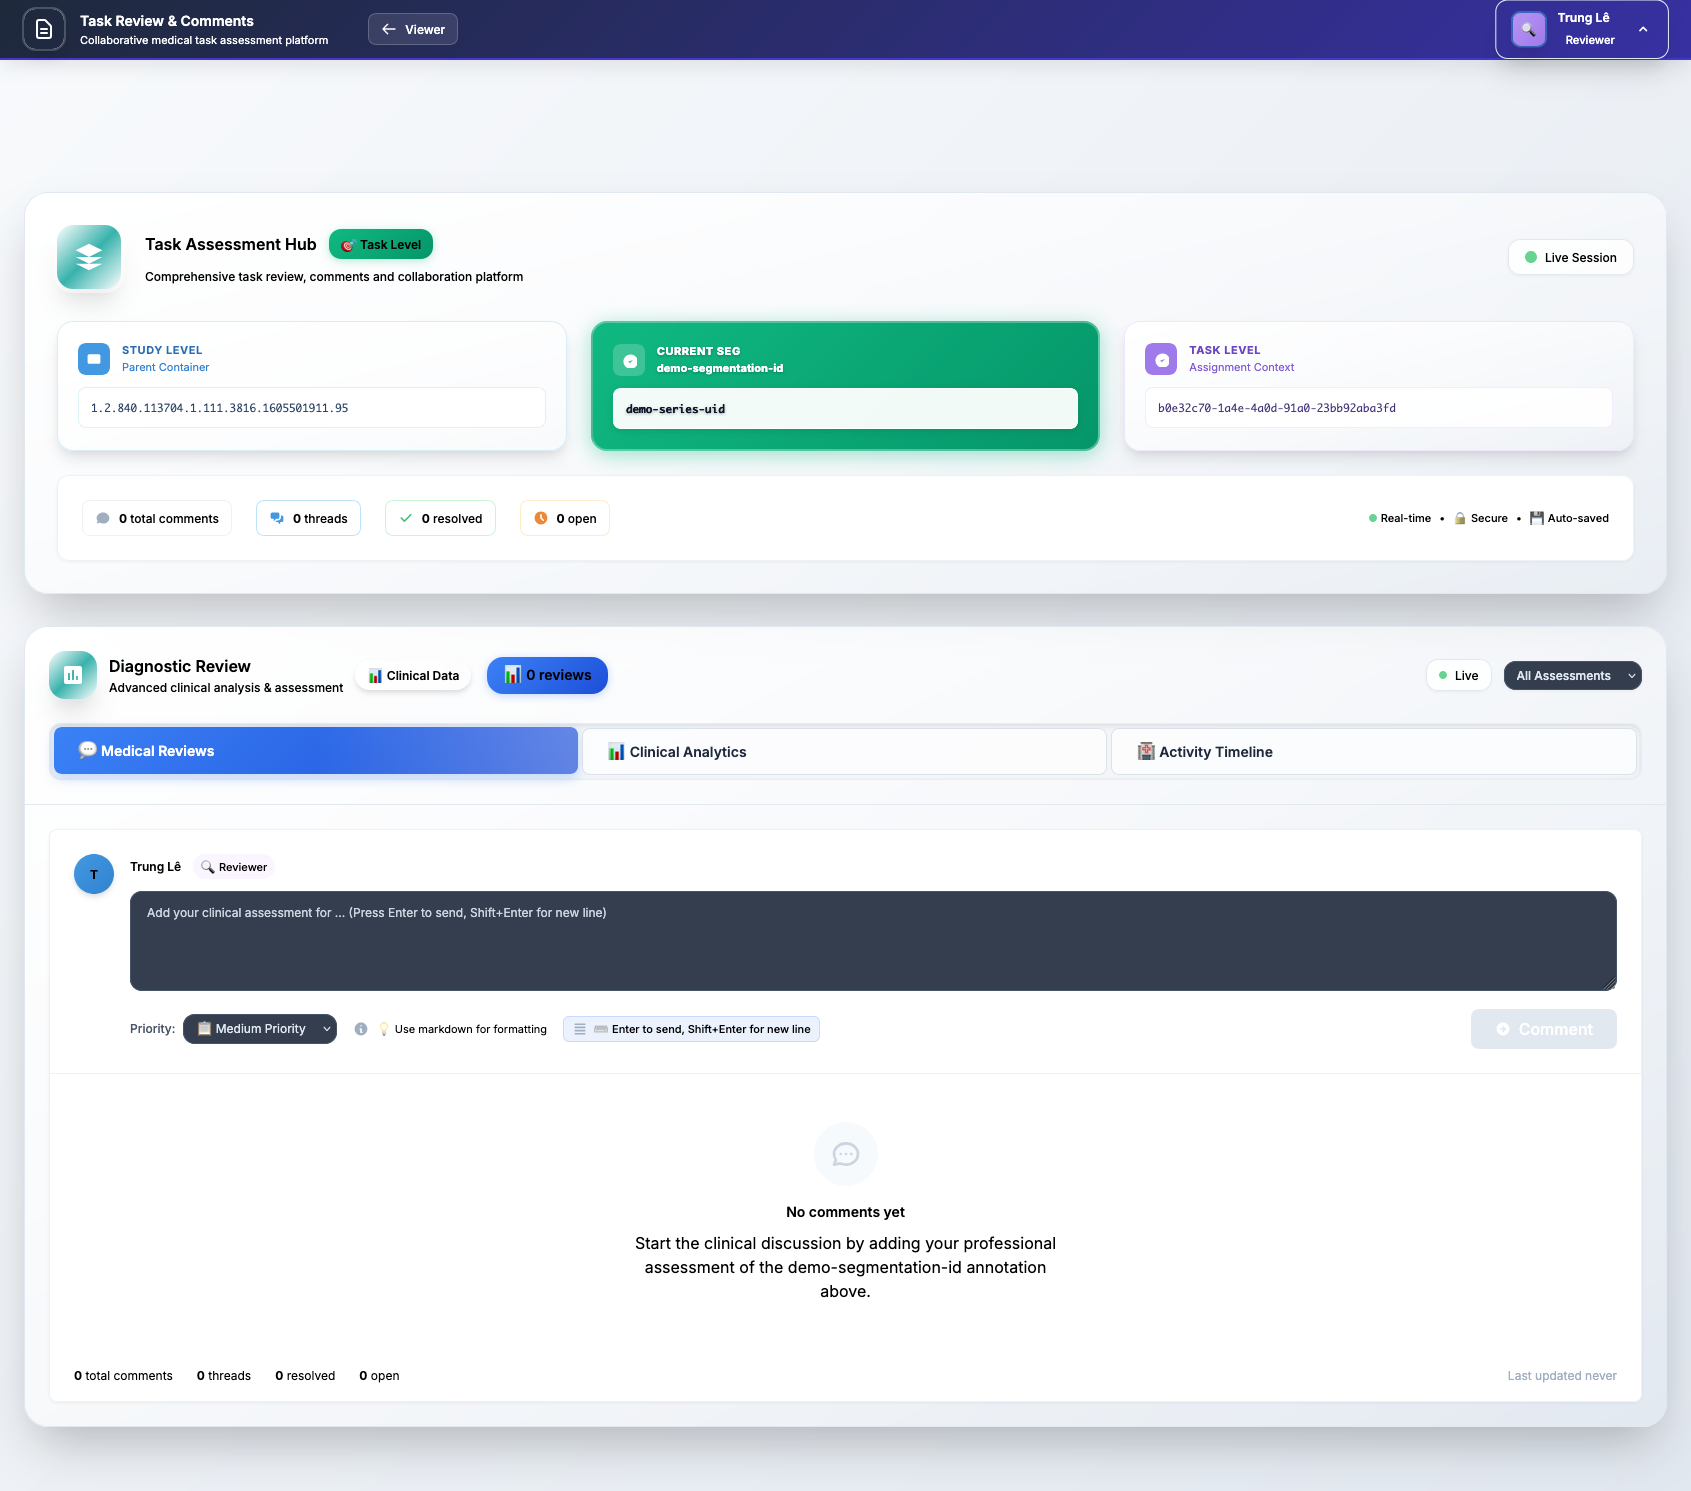
\includegraphics[width=1\textwidth]{content/resources/features/ohif comment.png}
    \caption{Task Assessment Hub with Annotation Commenting}
    \label{fig:annotation-comments}
\end{figure}

\subsubsection{Data Source Integration}
The system can connect to and ingest data items from external sources, including specialized medical imaging archives like Orthanc, streamlining the data acquisition process for annotation.

\begin{figure}[h!]
    \centering
    \includegraphics[width=1\textwidth]{content//resources//features//orthanc.png}
    \caption{Orthanc Data Source Integration Interface}
    \label{fig:orthanc-integration}
\end{figure}

\subsection{Backend Automation: Virtual Users and Cron-Based Workflow Orchestration}
A cornerstone of the platform's backend architecture is its capacity for automated workflow progression, reducing the need for direct human intervention in repetitive or system-driven tasks. This is achieved through a synergy of "virtual users" and scheduled cron jobs, forming an intelligent, SQL-based orchestration layer.

\subsubsection{The Concept of Virtual Users}
To manage automated, non-human operations, the system employs "virtual users." These are specialized user accounts within the `\_users` table, distinguished by an `is\_system` boolean field set to `true`. They act as system-level actors for specific automated functions, such as:
\begin{itemize}
    \item \textbf{START}: Initiates new tasks in a workflow.
    \item \textbf{ROUTER}: Manages conditional logic, directing tasks based on predefined rules embedded in workflow stage configurations.
    \item \textbf{CONSENSUS}: Orchestrates the aggregation and comparison of multiple annotations to determine agreement, critical for quality control.
\end{itemize}
When a task enters a stage requiring automated processing, it is assigned to one of these virtual users within the `\_task\_assignments` table, awaiting system action.

\subsubsection{Cron Jobs: The Automation Trigger}
Unlike human-initiated tasks, tasks assigned to virtual users are processed by scheduled cron jobs. These are PostgreSQL functions configured to execute at regular intervals (e.g., every minute), establishing a robust polling mechanism. Key cron jobs for workflow automation include `workflow\_start`, `workflow\_route`, `workflow\_consensus`, and `workflow\_consensus\_holding`.

\subsubsection{The Automated Orchestration Flow}
The automated workflow progresses through a clear, stateful sequence recorded within the database:
\begin{enumerate}
    \item \textbf{Assignment to Virtual User}: A task transitions to an automated stage (e.g., a `ROUTER` stage), triggering the creation of a new `\_task\_assignments` record that links the task to the stage and the relevant virtual user.
    \item \textbf{Scheduled Execution}: A periodically running cron job (e.g., `workflow\_route()`) is invoked.
    \item \textbf{Task Processing}: The executing function queries `\_task\_assignments` for all 'PENDING' tasks assigned to its corresponding virtual user.
    \item \textbf{Logic Execution}: For each pending task, the function executes specialized logic. For a `ROUTER` stage, this involves interpreting the `custom\_config` JSONB field from the `\_workflow\_stages` entry to determine the next path.
    \item \textbf{Workflow Progression}: Upon logic execution, the function advances the task to the next stage by:
    \begin{itemize}
        \item Updating the current assignment's status to 'COMPLETED'.
        \item Determining the subsequent stage ID using `on\_success\_stage\_id` or `on\_failure\_stage\_id`.
        \item Creating a new `\_task\_assignments` record for the next stage, assigning it to the appropriate human or virtual user. The `previous\_task\_assignment\_id` is linked to the completed assignment, ensuring an immutable and auditable event chain.
    \end{itemize}
\end{enumerate}
This cron-based approach establishes a powerful, asynchronous, and fully automated backend engine, driving the workflow forward in a serverless architecture.

\begin{figure}[h!]
    \centering
    % \includegraphics[width=0.8\textwidth]{path/to/your/workflow\_automation\_flow.png} % No specific image provided for this abstract concept.
    \caption{Conceptual Workflow Automation Flow}
    \label{fig:automation-flow}
\end{figure}

\subsection{Notifications}
A robust, built-in notification system ensures users are continuously informed about critical events and workflow updates.

\subsubsection{Event-Driven Notifications with Custom Payloads}
Users receive timely notifications for key events, such as new task assignments or actions requiring their attention. Each notification carries a custom payload, providing contextual data directly to the user, enhancing actionable information. Figure~\ref{fig:notifications} shows the notification panel, providing a chronological list of updates.

\begin{figure}[h!]
    \centering
    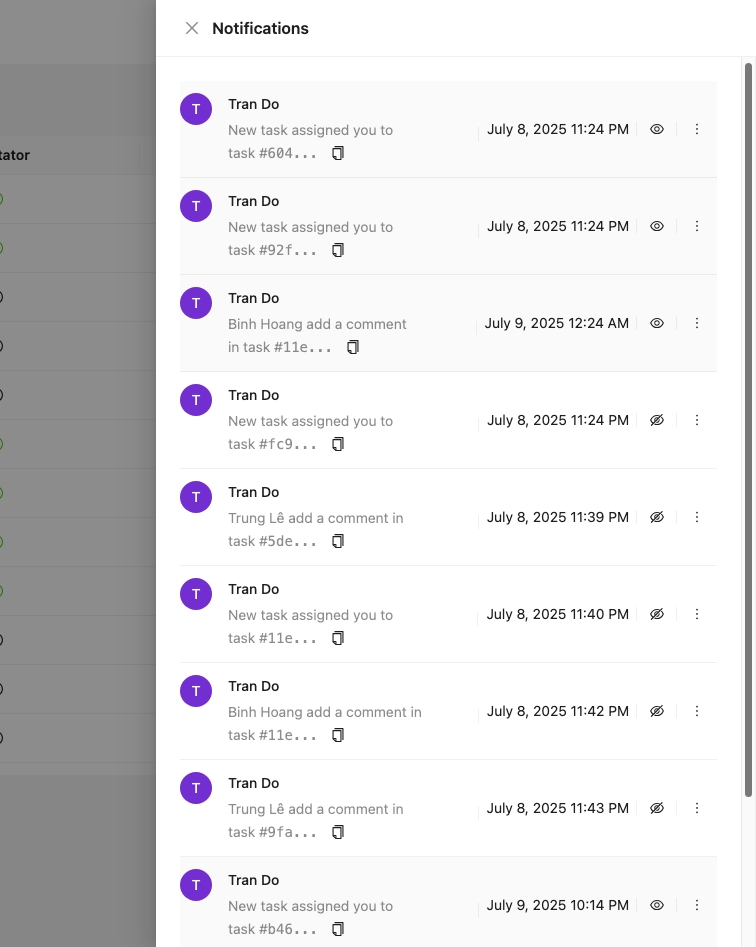
\includegraphics[width=0.6\textwidth]{content//resources//features//notifications.png}
    \caption{User Notification Panel}
    \label{fig:notifications}
\end{figure}

\subsubsection{View Tracking}
The system tracks notification viewing status, ensuring users do not miss critical updates and facilitating effective communication within the platform.

\subsection{System Integrations}
The platform is designed with extensibility in mind, allowing for seamless integration with external systems and machine learning models.

\subsubsection{Machine Learning Model Integration}
The system can connect to external ML models by storing their API endpoints. This capability enables advanced features such as model-assisted labeling (MITL), enhancing annotation efficiency and accuracy.
